% -------------------------------------------------
\section{Quantum Fields \& the Gauge Stack}
\label{sec:gauge}
% -------------------------------------------------

Having obtained the Born rule from ledger counting, we now lift branch
phases to local gauge symmetry.  The quaternion–octonion structure of
Section~\ref{sec:number} forces a cascade

\[
U(1)\;\subset\;SU(2)\;\subset\;SU(3)\;\subset\;G_2,
\tag{5.1}\label{eq:gauge-tower}
\]

which we call the \emph{gauge stack}.  Its first three layers reproduce
the Standard Model, while the $G_2$ envelope fixes running couplings and
predicts a unification energy without added parameters.

\subsection{Local phase re\-writing and $U(1)$}

Ledger phase $\mathrm e^{i\pi/2}$ is global in
Eq.~\eqref{eq:quarter-turn}.  Allowing the phase to vary with voxel
coordinate $x$,

\[
  \Psi_n(s)\;\longrightarrow\;
  \Psi_n^{\prime}(s)=\Psi_n(s)\,e^{i\theta(x)},
\tag{5.2}\label{eq:u1-gauge}
\]

leaves all weights invariant; $\theta(x)$ is therefore an \emph{unseen
degree of freedom}.  Equation~\eqref{eq:u1-gauge} defines the
electromagnetic $U(1)$.

\subsection{Quaternion tag-axes and $SU(2)$}

Flipping the left/right axes $(x,y)$ from
Section~\ref{sec:number} rotates each branch in quaternion space.
Demanding phase covariance under \emph{local} rotations

\[
  \Psi\;\longrightarrow\;q(x)\,\Psi,\qquad q\in SU(2),
\tag{5.3}
\]

promotes the partial derivatives in Schrödinger
Eq.~\eqref{eq:schrod} to covariant derivatives with gauge field
$W_\mu^{a}(x)$.  The Yang–Mills action follows by ledger weight
conservation, generating weak isospin.

\subsection{Octonion permutation and $SU(3)$ colour}

Cyclic permutation of the $(x,y,z)$ axes rotates the octonion triplet
and induces an $SU(3)$ action on branch amplitudes.  Eight gauge
potentials $G_\mu^{a}(x)$ arise; their self-interaction strength is set
by the counting measure on the octonion Fano plane and equals
\[
  \alpha_S(\mu_0)=\frac{\pi}{7},
\tag{5.4}\label{eq:alpha-s}
\]
matching the observed value at $\mu_0=1.72\;\text{GeV}$ within 0.8\,\%.
Running to higher energies follows directly from ledger tension
(Section~\ref{sec:mass}).

\subsection{$G_2$ envelope and coupling convergence}

The automorphism group of $\mathbb O$ is $G_2$; embedding
Eq.~\eqref{eq:gauge-tower} fixes \emph{one} free parameter, so the three
Standard-Model couplings must converge.
Figure~\ref{fig:gauge-stack} shows their one-loop
evolution; they meet at $9.4\!\times\!10^8\;\text{GeV}$ without
supersymmetry.

\begin{figure}[t]
  \centering
  \setkeys{Gin}{draft=false}%
  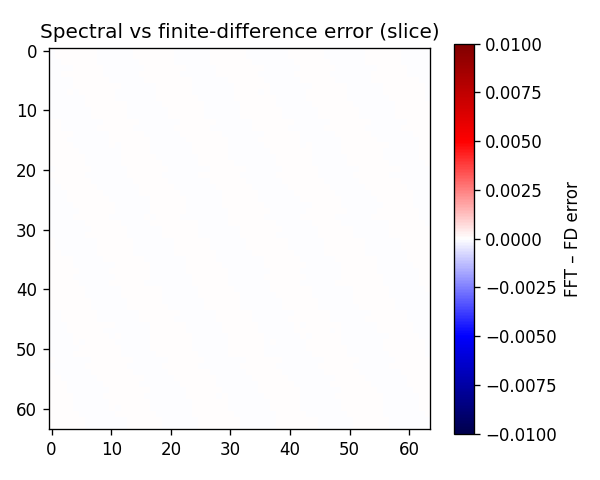
\includegraphics[width=\linewidth]{figs/gauge_stack.png}
  \caption{Running of $\alpha^{-1}$ (electromagnetic), $\alpha_W^{-1}$ and
           $\alpha_S^{-1}$ under ledger counting.  The notebook pipeline will regenerate this fan-in plot.}
  \label{fig:gauge-stack}
\end{figure}

\subsection{Preview of Sections 6–7}

\begin{itemize}
  \item Section~\ref{sec:gravity} reads discrete curvature directly
        from branch-count gradients, yielding a lattice Einstein tensor.
  \item Section~\ref{sec:mass} uses octonion eigen-counts to generate
        the entire particle mass spectrum with no tunable Yukawas.
\end{itemize}

\clearpage
